%%%%%%%%%%%%%%%%%%%%%%%%%%%%%%%%%%%%%%%%%
% Beamer Presentation
% LaTeX Template
% Version 1.0 (10/11/12)
%
% This template has been downloaded from:
% http://www.LaTeXTemplates.com
%
% License:
% CC BY-NC-SA 3.0 (http://creativecommons.org/licenses/by-nc-sa/3.0/)
%
%%%%%%%%%%%%%%%%%%%%%%%%%%%%%%%%%%%%%%%%%

%----------------------------------------------------------------------------------------
%   PACKAGES AND THEMES
%----------------------------------------------------------------------------------------

\documentclass{beamer}
\usepackage[encapsulated]{CJK}
\usepackage{CJKutf8}
\mode<presentation> {

% The Beamer class comes with a number of default slide themes
% which change the colors and layouts of slides. Below this is a list
% of all the themes, uncomment each in turn to see what they look like.

%\usetheme{default}
%\usetheme{AnnArbor}
%\usetheme{Antibes}
%\usetheme{Bergen}
%\usetheme{Berkeley}
%\usetheme{Berlin}
%\usetheme{Boadilla}
%\usetheme{CambridgeUS}
%\usetheme{Copenhagen}
%\usetheme{Darmstadt}
%\usetheme{Dresden}
%\usetheme{Frankfurt}
%\usetheme{Goettingen}
%\usetheme{Hannover}
%\usetheme{Ilmenau}
%\usetheme{JuanLesPins}
%\usetheme{Luebeck}
\usetheme{Boadilla}
%\usetheme{Malmoe}
%\usetheme{Marburg}
%\usetheme{Montpellier}
%\usetheme{PaloAlto}
%\usetheme{Pittsburgh}
%\usetheme{Rochester}
%\usetheme{Singapore}
%\usetheme{Szeged}
%\usetheme{Warsaw}

% As well as themes, the Beamer class has a number of color themes
% for any slide theme. Uncomment each of these in turn to see how it
% changes the colors of your current slide theme.

%\usecolortheme{albatross}
%\usecolortheme{beaver}
%\usecolortheme{beetle}
%\usecolortheme{crane}
%\usecolortheme{dolphin}
%\usecolortheme{dove}
%\usecolortheme{fly}
%\usecolortheme{lily}
%\usecolortheme{orchid}
%\usecolortheme{rose}
%\usecolortheme{seagull}
%\usecolortheme{seahorse}
%\usecolortheme{whale}
%\usecolortheme{wolverine}

%\setbeamertemplate{footline} % To remove the footer line in all slides uncomment this line
%\setbeamertemplate{footline}[page number] % To replace the footer line in all slides with a simple slide count uncomment this line

%\setbeamertemplate{navigation symbols}{} % To remove the navigation symbols from the bottom of all slides uncomment this line

\setbeamertemplate{footline}
{
\leavevmode%
  \hbox{%
  \begin{beamercolorbox}[wd=1\paperwidth,ht=2.25ex,dp=1ex,right]{date in head/foot}%
    \insertframenumber{} / \inserttotalframenumber\hspace*{2ex}
  \end{beamercolorbox}
}%
  \vskip0pt%
}

}

\usepackage{graphicx} % Allows including images
\usepackage{booktabs} % Allows the use of \toprule, \midrule and \bottomrule in tables

%----------------------------------------------------------------------------------------
%   TITLE PAGE
%----------------------------------------------------------------------------------------





\title {Open Platform Software Final Project}

\author{Group 11} % Your name
\institute[UCLA] % Your institution as it will appear on the bottom of every slide, may be shorthand to save space
{

1041411 朱昆毅\\
1041427 李家賢\\
1041428 呂宜叡\\
1041429 王俊傑\\
1041448 陳冠穎\\ % Your institution for the title page


\medskip
\textit{} % Your email address
}
\date{June 22, 2018} % Date, can be changed to a custom date

\begin{document}
\begin{CJK}{UTF8}{bsmi}
\begin{frame}
\titlepage % Print the title page as the first slide
\end{frame}



\begin{frame}
\frametitle{} % Table of contents slide, comment this block out to remove it
\begin{figure}

\includegraphics[width=0.5\linewidth]{logo.jpg}

\end{figure}
\end{frame}

\begin{frame}
\frametitle{} % Table of contents slide, comment this block out to remove it
\begin{figure}
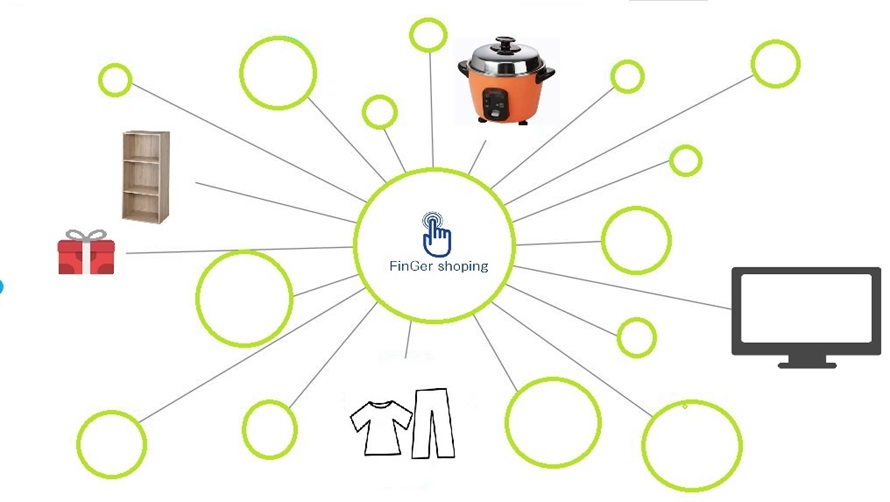
\includegraphics[width=1\linewidth]{test.jpg}
Provide online trading platform
\end{figure}
\end{frame}

%----------------------------------------------------------------------------------------
%   PRESENTATION SLIDES
%----------------------------------------------------------------------------------------

%------------------------------------------------
\section{First Section} % Sections can be created in order to organize your presentation into discrete blocks, all sections and subsections are automatically printed in the table of contents as an overview of the talk
%------------------------------------------------

\subsection{Subsection Example} % A subsection can be created just before a set of slides with a common theme to further break down your presentation into chunks

\begin{frame}
\frametitle{The Intelligent Communication}
\begin{figure}

\includegraphics[width=0.8\linewidth]{human.jpg}
\end{figure}
\begin{center}
Human to Human
\end{center}

\end{frame}

%------------------------------------------------

\begin{frame}
\frametitle{Why you need FinGer ?}

\begin{columns}[c]
\column{.45\textwidth}
\textbf{}
\begin{enumerate}
\item Anytime, anywhere
\item Immediate notification
\item Simple implementation
\end{enumerate}

\column{.5\textwidth}

\begin{figure}

\includegraphics[width=0.4\linewidth]{car.jpg}
\end{figure}

\end{columns}


\end{frame}

%------------------------------------------------

\begin{frame}
\frametitle{Why you need FinGer ?}

\begin{figure}
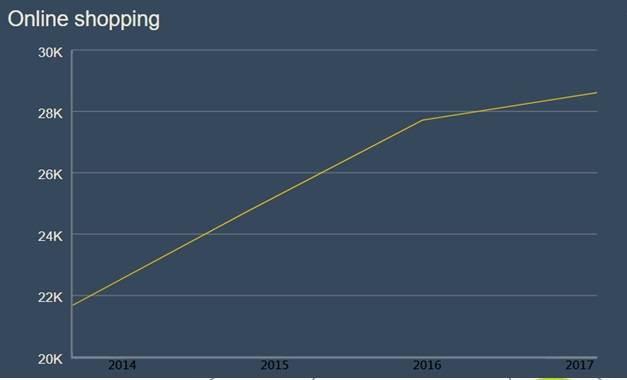
\includegraphics[width=0.8\linewidth]{online.jpg}
\end{figure}
\begin{center}
The Probability for Online trading
\end{center}

\end{frame}

%------------------------------------------------

\begin{frame}
\frametitle{Features Of FinGer}

\begin{figure}
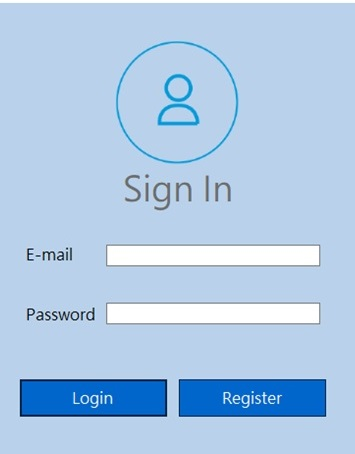
\includegraphics[width=0.4\linewidth]{signin.jpg}
\end{figure}

\end{frame}

%------------------------------------------------
\section{Second Section}
%------------------------------------------------

\begin{frame}
\frametitle{Features Of FinGer}
\begin{columns}[c]
\column{.45\textwidth}
\textbf{}
\begin{enumerate}
\item Search system
\end{enumerate}

\column{.5\textwidth}

\begin{figure}
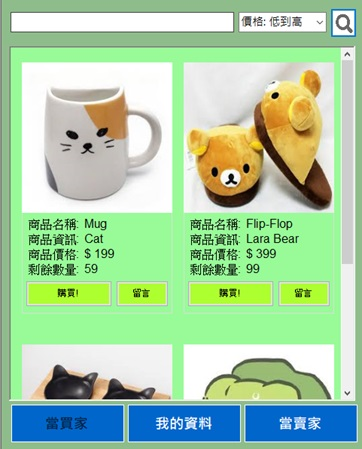
\includegraphics[width=0.6\linewidth]{search.jpg}
\end{figure}

\end{columns}

\end{frame}

%------------------------------------------------

\begin{frame}
\frametitle{Features Of FinGer}
\begin{columns}[c]
\column{.45\textwidth}
\textbf{}
\begin{enumerate}
\item Message area for communication
\item Grading System
\end{enumerate}

\column{.5\textwidth}

\begin{figure}
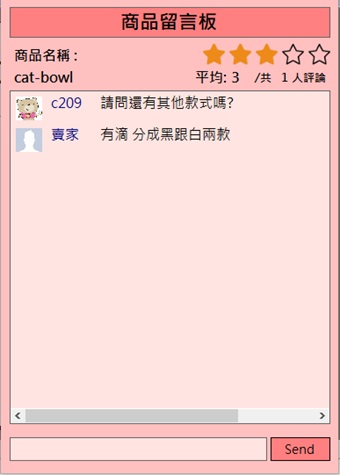
\includegraphics[width=0.6\linewidth]{star.jpg}
\end{figure}

\end{columns}

\end{frame}

%------------------------------------------------

\begin{frame}
\frametitle{Features Of FinGer}
\begin{columns}[c]
\column{.45\textwidth}
\textbf{}
\begin{enumerate}
\item Immediate notice
\item Sales record
\vspace{10pt}

\begin{figure}
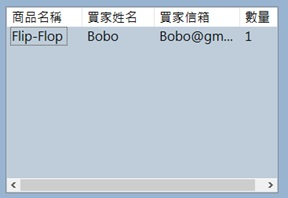
\includegraphics[width=0.5\linewidth]{record.jpg}
\end{figure}
\end{enumerate}

\column{.5\textwidth}

\begin{figure}
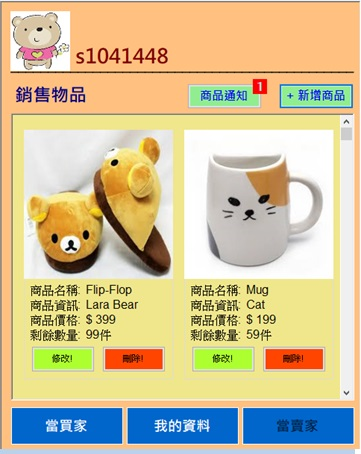
\includegraphics[width=0.6\linewidth]{note.jpg}
\end{figure}

\end{columns}

\end{frame}

%------------------------------------------------

\begin{frame}
\begin{figure}

\includegraphics[width=0.3\linewidth]{logo.jpg}
\end{figure}
\begin{figure}

\includegraphics[width=0.7\linewidth]{good.jpg}
\end{figure}
\end{frame}

%------------------------------------------------



%------------------------------------------------



%------------------------------------------------

\begin{frame}
\Huge{\centerline{Demo}}
\end{frame}

%----------------------------------------------------------------------------------------
\end{CJK}
\end{document}